\documentclass[18pt]{amsart}
\usepackage{geometry}                % See geometry.pdf to learn the layout options. There are lots.
\geometry{letterpaper}                   % ... or a4paper or a5paper or ... 
%\geometry{landscape}                % Activate for for rotated page geometry
%\usepackage[parfill]{parskip}    % Activate to begin paragraphs with an empty line rather than an indent
\usepackage{graphicx}
\usepackage{amssymb}
\usepackage{epstopdf}
\usepackage{fullpage}

%\oddsidemargin -0.5in
%\topmargin -0.5in
%\textheight 9.75in


\DeclareGraphicsRule{.tif}{png}{.png}{`convert #1 `dirname #1`/`basename #1 .tif`.png}

\title{Brief Article}
\author{The Author}
%\date{}                                           % Activate to display a given date or no date

\thispagestyle{empty}
\begin{document}
%\maketitle
%\section{}
%\subsection{}
{
\huge
\begin{center}
\begin{tabular}{c}
\textsc{CMP 108:  Programming for Data Analysis}\\
\\
\\

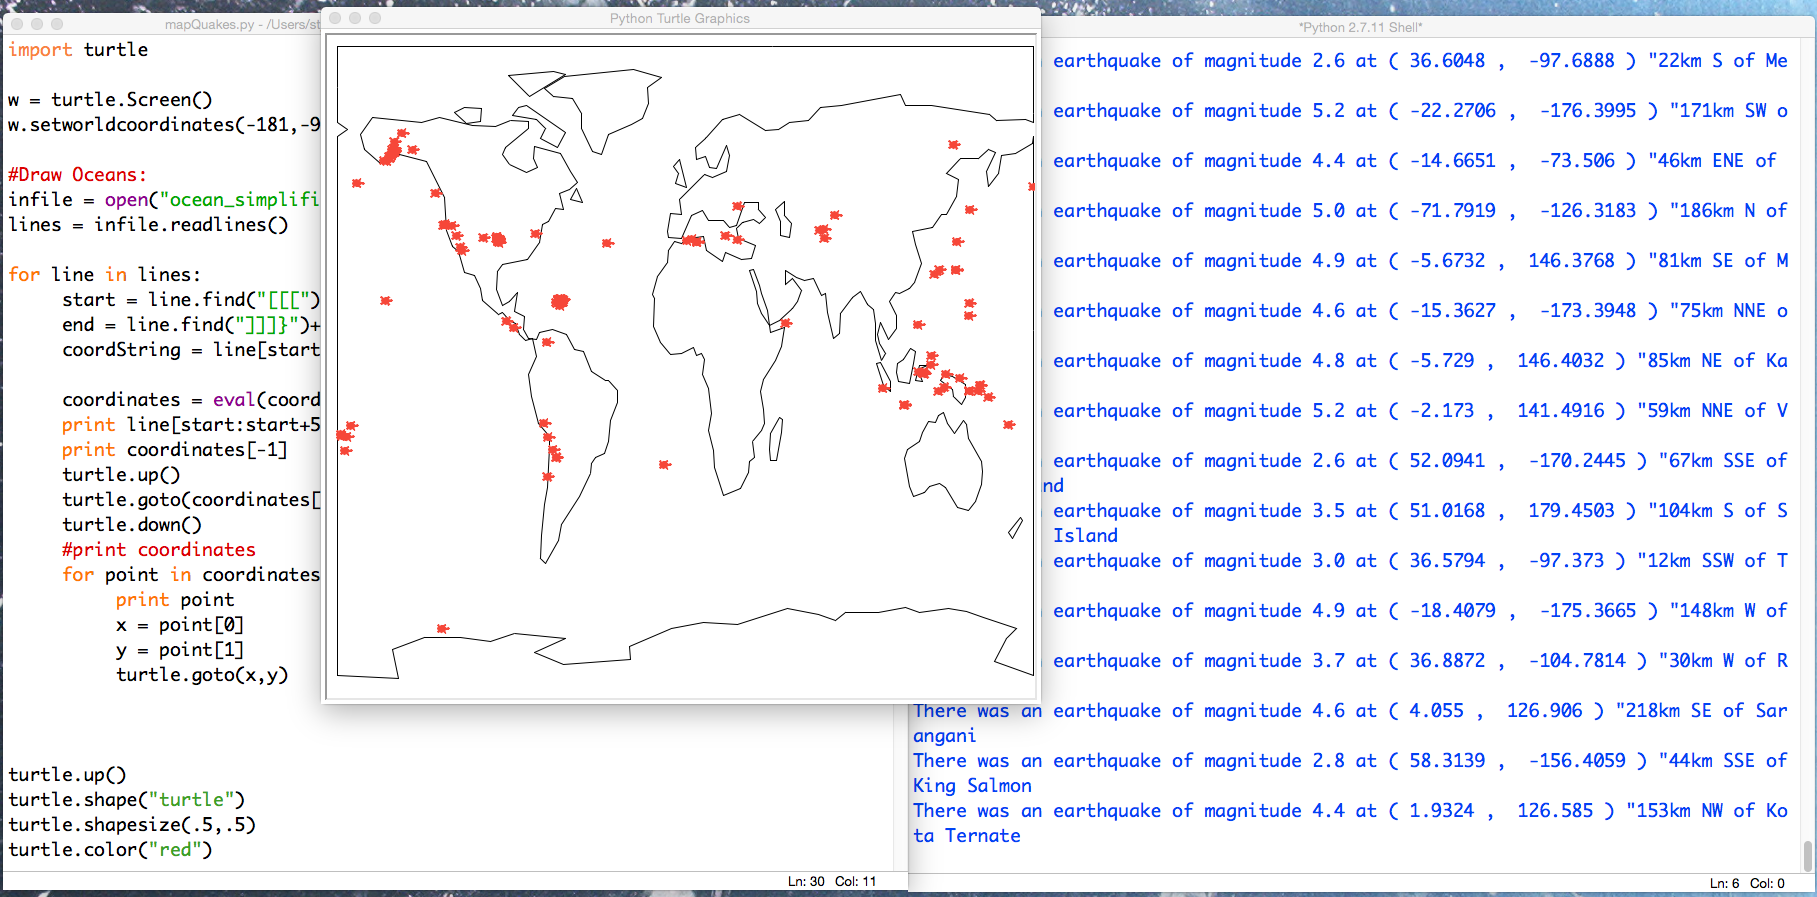
\includegraphics[width=6.25in]{mappingQuakeData.png}\\
{\tiny (Quake data from US Geological Survey live feed.)}\\
\\


\end{tabular}
\end{center}

{%\LARGE
\begin{itemize}
	\item Hands-on course for analyzing and visualizing big data sets.
	\item Learn the popular Python programming language. % and packages to analyze \& visualize results.
	\item Learn R and related statistics techniques.	
	\item Design \& build a real world data project for your jobs portfolio.		
	\vspace{.1in}
	\item No previous programming background needed.
	\item Designed for students not majoring in computer science\\
	 (future computer science majors should take CMP 167).
	\vspace{.2875in}
	\item Lectures on Wednesdays at 1:50-3:30pm;\\ 
	Lab sections available on Monday or Wednesday afternoons.
	\item {\em Register on CUNY First.  E-permit students welcome.}
	\item {\em More information at:} {\tt\Large comet.lehman.cuny.edu/stjohn/teaching/cmp108}.
\end{itemize}
}

\vspace{.125in}
\begin{center}
{\footnotesize Lehman College $\bullet$ City University of New York $\bullet$ Spring 2017}
\end{center}
\end{document}  